


%----------------------------------------------------------------------------------------
%\documentclass[a4paper,fleqn,twocolumn]{article} 
\documentclass[11pt]{article}

\usepackage{lipsum} % Package to generate dummy text throughout this template

\usepackage[sc]{mathpazo} % Use the Palatino font
\usepackage[T1]{fontenc} % Use 8-bit encoding that has 256 glyphs
\linespread{1.05} % Line spacing - Palatino needs more space between lines
\usepackage{microtype} % Slightly tweak font spacing for aesthetics

\usepackage[hmarginratio=1:1,top=32mm,columnsep=20pt]{geometry} % Document margins
\usepackage{multicol} % Used for the two-column layout of the document
\usepackage{hyperref} % For hyperlinks in the PDF

\usepackage[hang, small,labelfont=bf,up,textfont=it,up]{caption} % Custom captions under/above floats in tables or figures
\usepackage{booktabs} % Horizontal rules in tables
\usepackage{float} % Required for tables and figures in the multi-column environment - they need to be placed in specific locations with the [H] (e.g. \begin{table}[H])
\usepackage[ngerman, english]{babel}
\usepackage{lettrine} % The lettrine is the first enlarged letter at the beginning of the text
\usepackage{paralist} % Used for the compactitem environment which makes bullet points with less space between them
\usepackage{floatflt}
\usepackage{abstract} % Allows abstract customization
\renewcommand{\abstractnamefont}{\normalfont\bfseries} % Set the "Abstract" text to bold
\renewcommand{\abstracttextfont}{\normalfont\small\itshape} % Set the abstract itself to small italic text

\usepackage{titlesec} % Allows customization of titles
%\renewcommand\thesection{\Roman{section}}
\titleformat{\section}[block]{\large\scshape\centering}{\thesection.}{1em}{} % Change the look of the section titles
\usepackage{graphicx}
\usepackage{fancyhdr} % Headers and footers
\pagestyle{fancy} % All pages have headers and footers
\fancyhead{} % Blank out the default header
\fancyfoot{} % Blank out the default footer
%\fancyhead[C]{On street parkling$\bullet$ February 2013 $\bullet$ Vol. I, No. 1} % Custom header text
\fancyfoot[RO,LE]{\thepage} % Custom footer text

\usepackage{listings}
\usepackage{acronym}

%----------------------------------------------------------------------------------------
%	TITLE SECTION
%----------------------------------------------------------------------------------------
\begin{document}



\title{\vspace{40mm}\fontsize{24pt}{10pt}\selectfont\textbf{Project Work\\NFC Microcontroller / Smartphone Bluetooth Device}} % Article title

\author{
\large
\textsc{Andreas Sauter} \\ % Your name
\textsc{Mtr-Nr: 747830} \\ % Your name
\textsc{Hochschule Esslingen} \\ % Your institution
\normalsize 
\href{mailto:ansags03@hs-esslingen.de}{ansags03@hs-esslingen.de}\\ % Your email address

\textsc{Project supervisor: Vikas Agrawal}
\vspace{2mm}
}

\date{\today}


\begin{figure}
 \centering
 
\includegraphics [width=10cm]{HE_Logo_4c.pdf} 
\end{figure}

%----------------------------------------------------------------------------------------


\maketitle % Insert title

\thispagestyle{empty}
\newpage

%----------------------------------------------------------------------------------------
%	CONTENT
%----------------------------------------------------------------------------------------

\thispagestyle{fancy} % All pages have headers and footers
\setcounter{page}{1} 
\tableofcontents


%---------------------------------------------------- New Page -------------------------------------------------
\newpage

\begin{acronym}
 \acro{NFC}{Near Field Communication}
 \acro{RFID}{Radio Frequent Identification}
 \acro{ASK}{Amplitude Shift Keying}
 \acro{FSK}{Frequency Shift Keying}
 \acro{PSK}{Phase Shift Keying}
 \acro{EDR}{Enhanced Data Rate}
\end{acronym}


%---------------------------------------------------- New Page -------------------------------------------------
\newpage


\thispagestyle{fancy} % All pages have headers and footers



\section{NFC Microcontroller Project}

This chapter will provide basic information of the Near Field Communication (= NFC). There will also be an explanation of how to
setup the tools and hardware of the microcontroller and debugger to run this project, as well as an explanation of the running source code and MAKE file.

\begin{figure}[H]

 \centering
 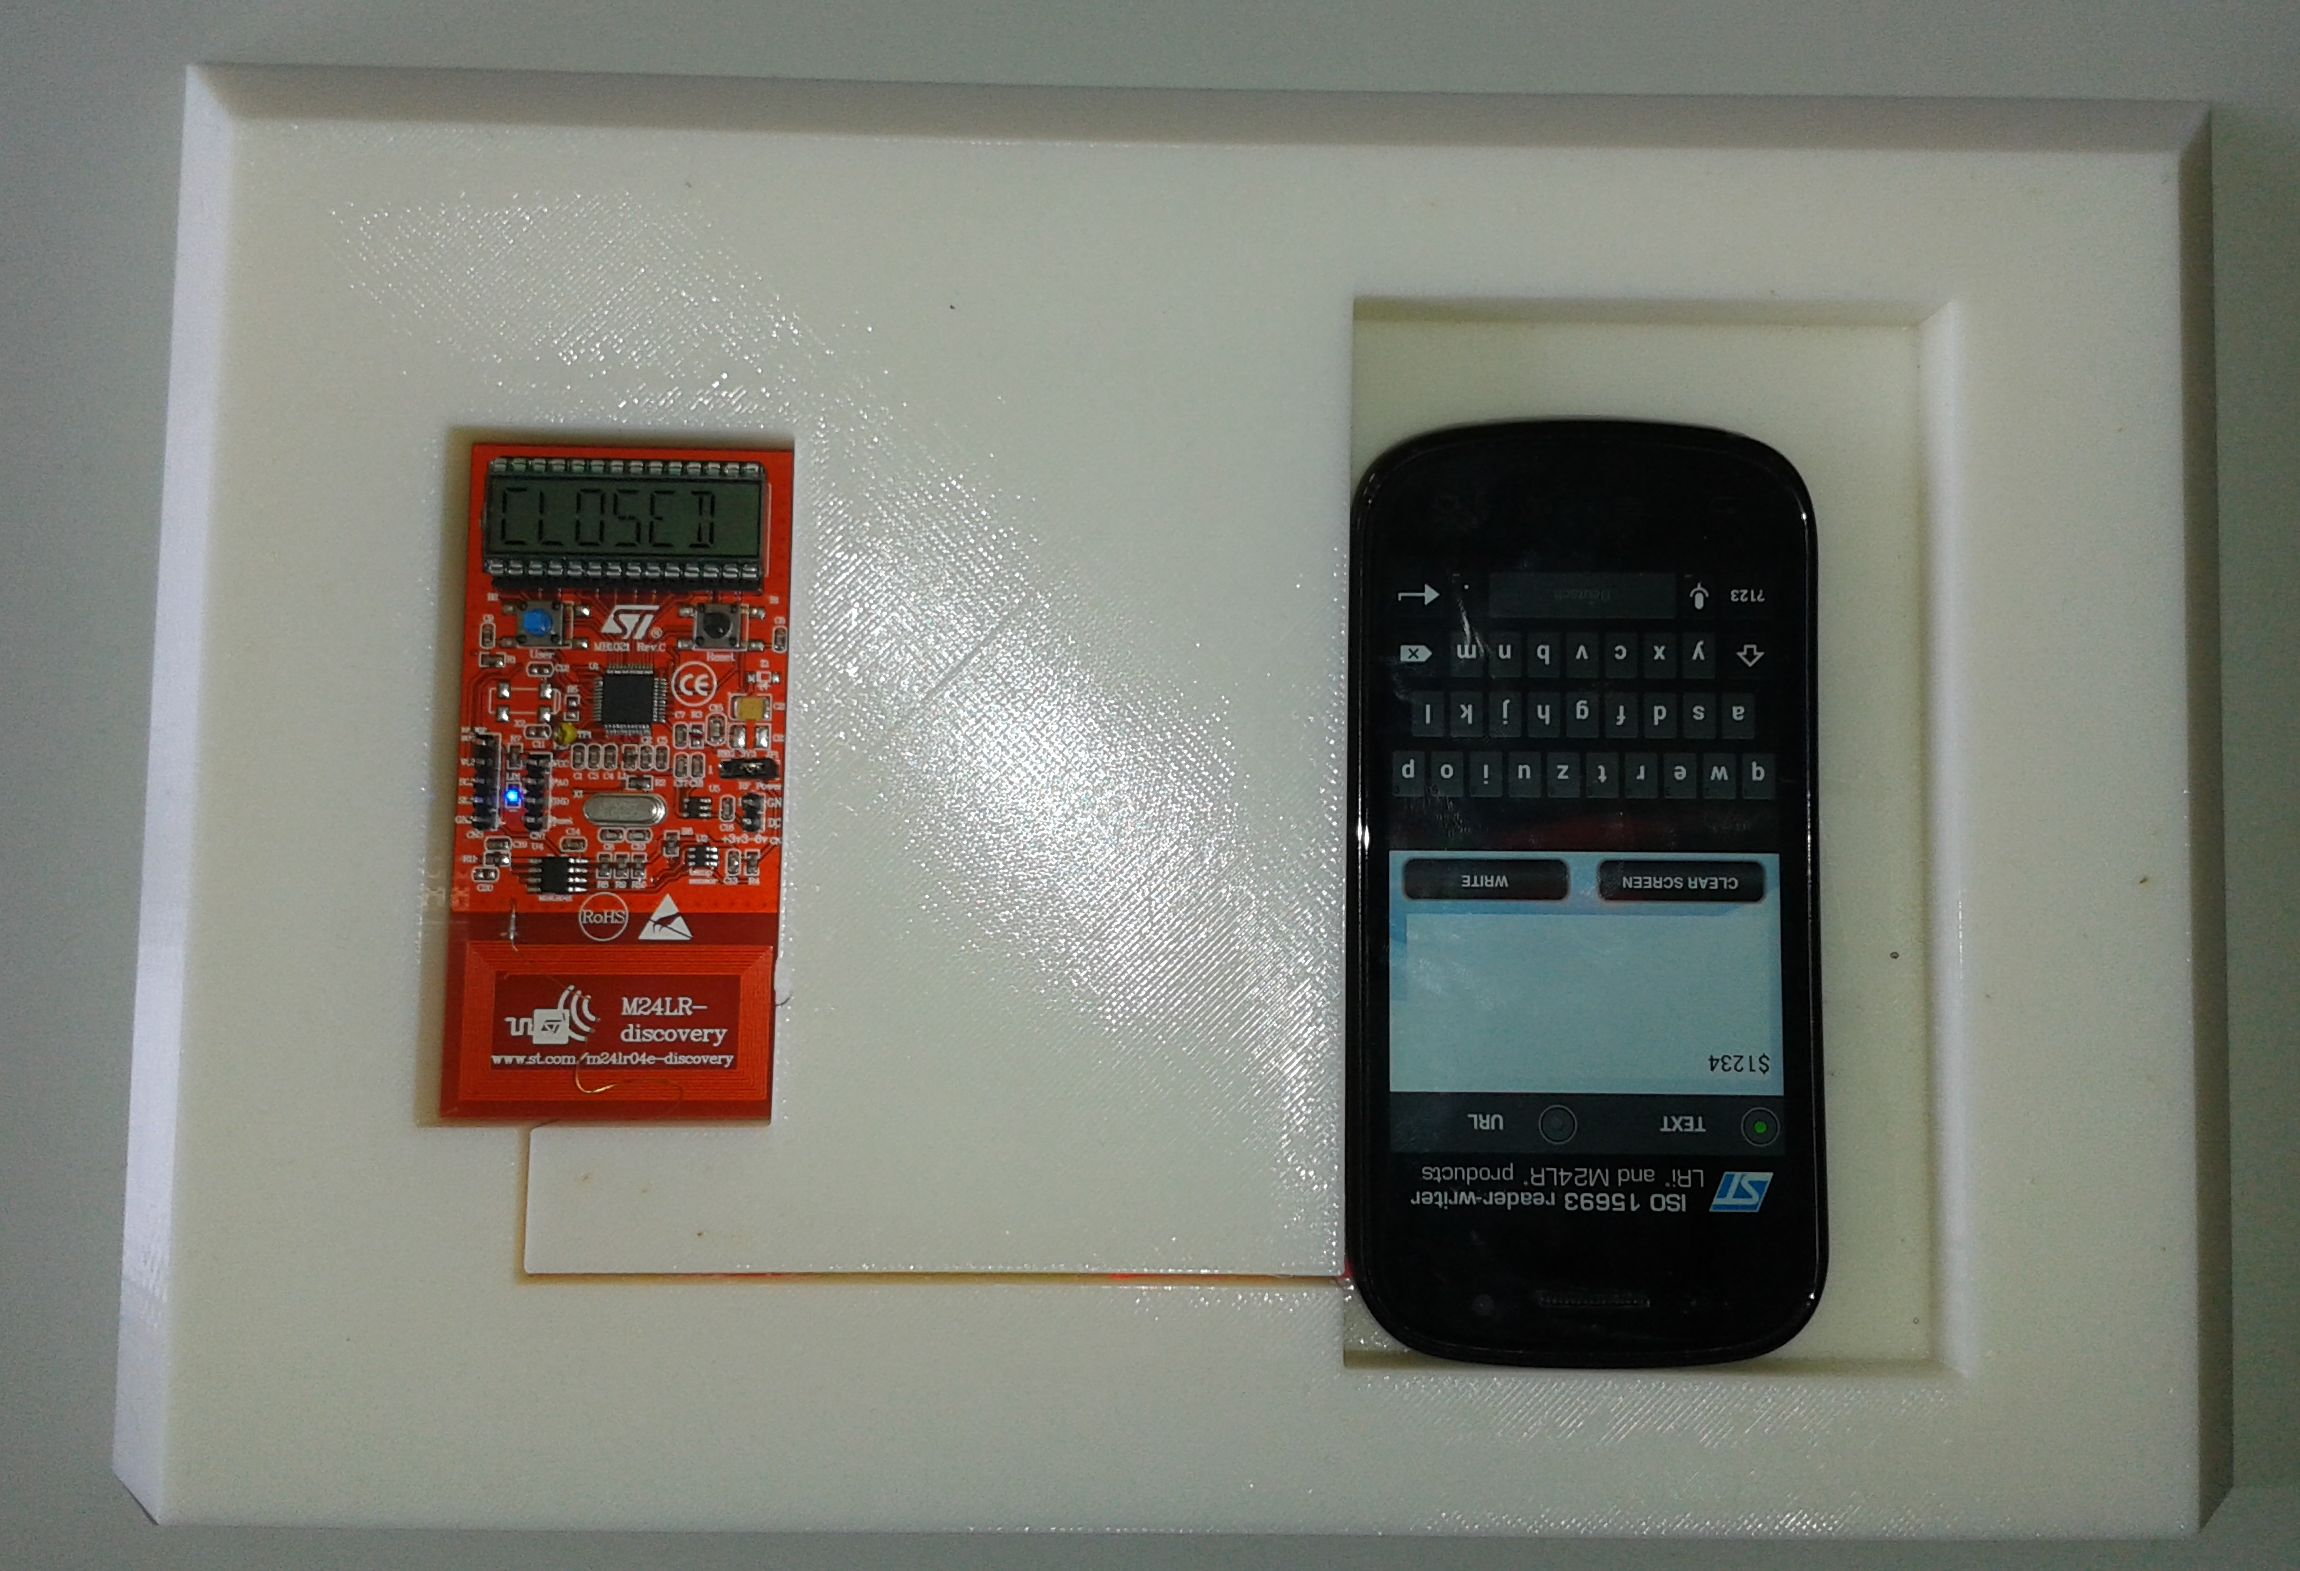
\includegraphics [width=16cm]{NFCProject.jpg}
\end{figure}


%---------------------------------------------------- New Page -------------------------------------------------
\newpage
\subsection{Near Field Communication}

The "`Near Field Communication"' (NFC) is a set of standards to establish a radio communication of two devices by bringing them into close range to each other.
It is based on the technology of Radio Frequent Identification (RFID) and includes the standards ISO/IEC 18092 and those defined by the NFC Forum, which consists of
companies of the electronic industry, such as Intel, Google, Nokia, Samsung, Sony, Infineon, LG and Texas Instruments\cite{cite2}.
NFC can be used to provide contactless transactions, data exchange and setup of Wi-Fi or Bluetooth connections.\cite{cite1}

\subsubsection{Technology of NFC}

The data exchange of two NFC devices is done by electromagnetic waves. Therefor each device needs a NFC antenna which is build with the principles of a coil. In smartphones there is mostly used an antenna with N=4 windings as it can be seen at the image of the NFC antenna of the Galaxy Nexus S below.

\begin{figure}[H]

 \centering
 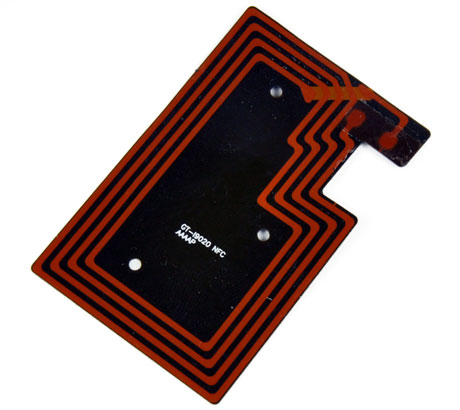
\includegraphics [width=7cm]{nexus-s-nfc-antenna.jpg} % You can use this if the picture is in the same folder as the .tex file. Otherwise see above
 \caption{NFC antenna of Google Nexus S\cite{cite3}}
\end{figure}


NFC is using a frequency range of 13.56 MHz and provides bitrates between 106 kbit/s to 424 kbit/s for data exchange. Compared with the RFID, where the active and passive device has to be chosen before, with the use of NFC the active and passive device can change all the time.
The coupling of NFC devices is done by inductivity. This leads to the possibility to power up passive components wihtout an energy supply. For example a smartphone can be used to power up a NFC tag (description and how to use NFC tags follows in chapter X) and then start exchanging the stored data.

There are two different communication modes:

\begin{itemize} 
\item Passive communication mode: The initiator device provides a carrier field and the target device answers by modulating the existing field. In this mode, the target device may draw its operating power from the initiator-provided electromagnetic field, thus making the target device a transponder.
\item Active communication mode: Both initiator and target device communicate by alternately generating their own fields. A device deactivates its RF field while it is waiting for data. In this mode, both devices typically have power supplies.
\end{itemize} 

\begin{figure}[H]

 \centering
 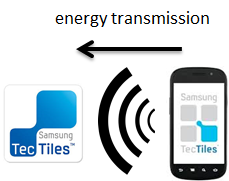
\includegraphics [width=7cm]{smartphone_nfctag.png} % You can use this if the picture is in the same folder as the .tex file. Otherwise see above
 \caption{Energy transmission with NFC}
\end{figure}

However if both NFC devices have an external power supply the distance between both devices can be larger than using one device with and one device without an external power supply.

\subsubsection{Data Transmission}

As mentioned above NFC uses a sine wave with a frequency of 13.56 MHz to transmit data. For the duplex mode, NFC uses the half duplex. This means that there is steadily a transmission of waves, which can also be used to power up a NFC device. But the transmission of data can only take place by one device at a time. The image below shows such a half duplex mode. The yellow bar is the steady transmission of a wave, the red bar is showing one device and the orange bar the other device.

\begin{figure}[H]

 \centering
 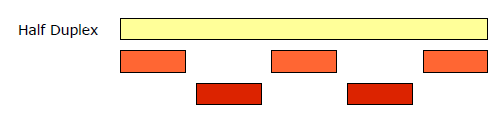
\includegraphics [width=7cm]{HalfDuplex.png} % You can use this if the picture is in the same folder as the .tex file. Otherwise see above
 \caption{Half duplex mode\cite{cite4}}
\end{figure}

To distinguish between the digital values of 0 and 1, NFC uses the so called "`Amplitude Shift Keying"' (=ASK). This means that there will always be a amplitude of the sine wave greater than 0, but with different values for 0 and 1. While the digital 1 is transmitted with the maximum amplitude of the sine wave, the digital value of 0 is transmitted with an amplitude of about 90\% of the maximum value of the sine wave.

\begin{figure}[H]

 \centering
 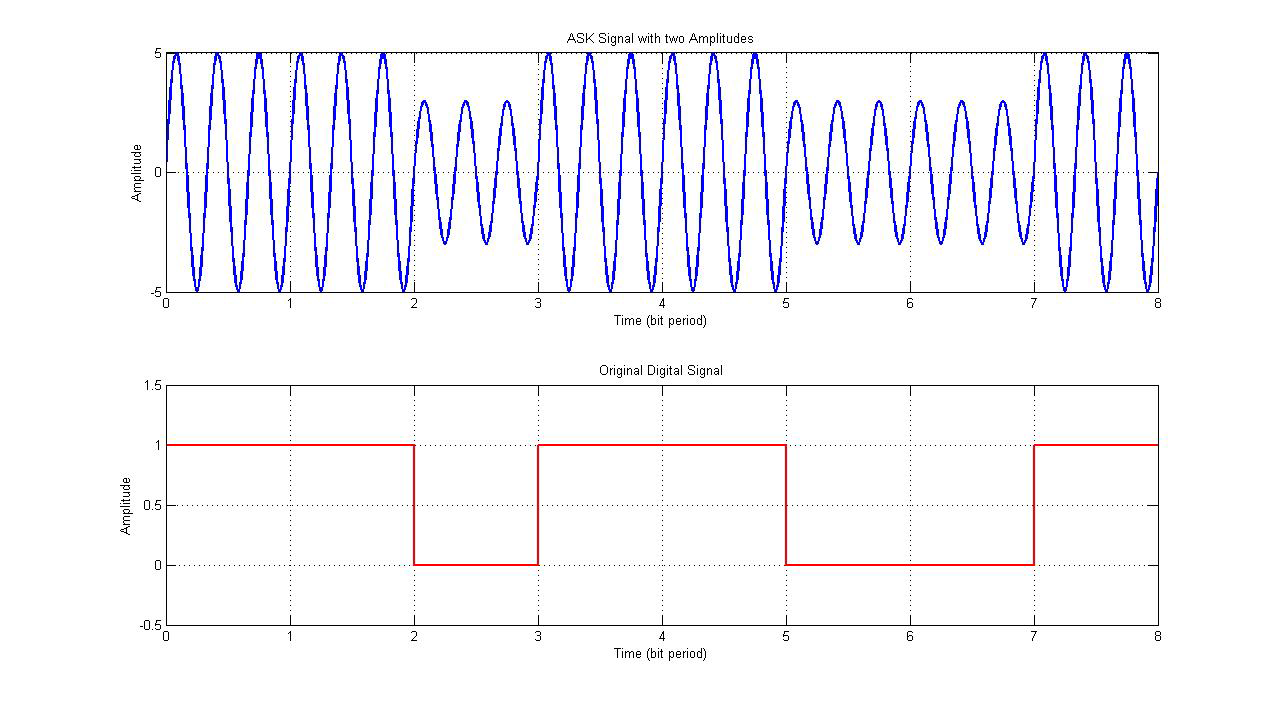
\includegraphics [width=15cm]{ASK.png} % You can use this if the picture is in the same folder as the .tex file. Otherwise see above
 \caption{Amplitude Shift Keying\cite{cite5}}
\end{figure}

Although NFC uses a frequency range of 13.56 MHz, because of the usage of the ASK there is only a bitrate between between 106 kbit/s to 424 kbit/s possible. This is due to the fact that you need more than one period of the sine wave to ensure that the wanted digital value is really meant to be sent.\\


\subsubsection{NFC Tags}

NFC Tags are small NFC antennas which can be used to store specific data. They use the passive communication mode, which means that the power comes from the other NFC device (e.g. smartphone). The data which can be stored on these tags can be among other things a simple plain text, a command to start a smartphone application or a command to start a bluetooth connection and pair with a specific device. In this project we use the NFC Tags from Samsung, which are called "`Samsung Tec Tiles"'. These NFC tags have a memory of 1KByte.

\begin{figure}[H]

 \centering
 
\includegraphics [width=3cm]{SamsungTecTiles.jpg} % You can use this if the picture is in the same folder as the .tex file. Otherwise see above
 \caption{Samsung Tec Tiles\cite{cite6}}
\end{figure}


\subsubsection{Sending Message to Microcontroller}
To send messages to the microcontroller in this project an android app called "`NFC-V Reader"' from the company ST Microelectronics is used. With this app it is possible to read or write NFC messages. The app icon looks like this:

\begin{figure}[H]
 \centering
 
\includegraphics [width=2cm]{nfcvreader.jpg} 
 \caption{NFC-V Reader Android App\cite{cite10}}
\end{figure}

To be able to send a message you have to first place a device with a NFC antenna next to the antenna of the smartphone. So after you start the app you will get the following screen :

\begin{figure}[H]
 \centering
 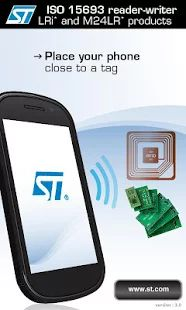
\includegraphics [width=3cm]{NFCvreader_place.jpg} 
 \caption{NFC-V Reader Android App\cite{cite10}}
\end{figure}

So after you put the smartphone on the antenna of the M24LR board you will get some information provided by the app with the following screen:

\begin{figure}[H]
 \centering
 \includegraphics [width=3cm]{NFCvreader_screen2.jpg} 
 \caption{NFC-V Reader Android App\cite{cite10}}
\end{figure}

So after to that click on the button "`NDEF FUNCTION"' to get to the next screen. Here you can now choose between reading or sending NFC messages. In this project you only have to send messages so click on the button "`WRITE NDEF MESSAGE"':

\begin{figure}[H]
 \centering
 \includegraphics [width=3cm]{NFCvreader_screen3.jpg} 
 \caption{NFC-V Reader Android App\cite{cite10}}
\end{figure}

After that you can enter the text you want to send to the microcontroller. In this project you send a pin number to the microcontroller to unlock it. The pin number has to start with a "`\$"' followed by 4 digits of numbers.

\begin{figure}[H]
 \centering
 \includegraphics [width=3cm]{NFCvreader_screen4.jpg} 
 \caption{NFC-V Reader Android App\cite{cite10}}
\end{figure}

\newpage 

\subsection{Microcontroller}

In this project the microcontroller M24LR from STMicroelectronics is used. It is a 8-bit microcontroller with 8 Kbytes of Flash memory and a small LCD display. It also has 4 Kbits of EEPROM and a I2C bus. Additionally there is a NFC antenna on the board, which is connected to an EEPROM memory chip. The data received by the NFC antenna is first stored in the NFC EEPROM and then send to microcontroller EEPROM via the I2C bus.

\begin{figure}[H]

 \centering
 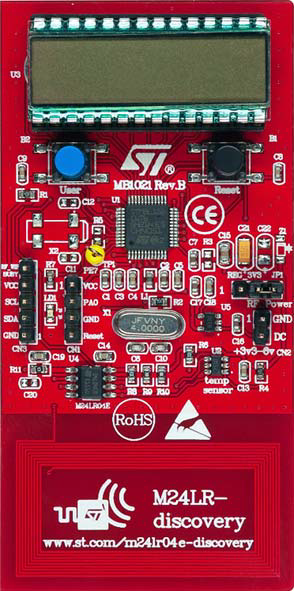
\includegraphics [width=2cm]{M24LRboard.png} 
 \caption{M24LR board\cite{cite7}}
\end{figure}

%-Picture of Microcontroller\\
\subsubsection{How to setup the hardware}
There are different ways to power the M24LR board. To change the power supply mode you have to set a jumper at a specific location of the board. This is shown in the next image:

\begin{figure}[H]

 \centering
 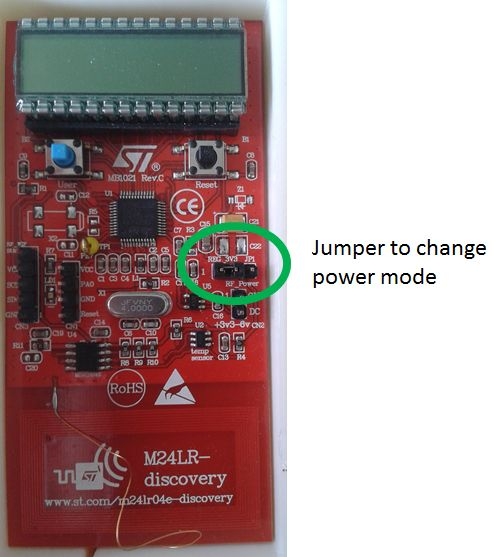
\includegraphics [width=6cm]{jumper.jpg} 
 \caption{M24LR board jumper position}
\end{figure}

One way to power the board is to use the energy of the smartphone that is produced by inductivity of the coil like antenna. Therefor the jumper has to be positioned so that "`RF\_Power"' and "`JP1"' are connected:

\begin{figure}[H]

 \centering
 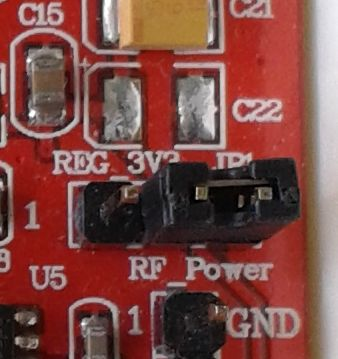
\includegraphics [width=4cm]{jumper_passive.jpg} 
 \caption{M24LR board jumper position}
\end{figure}

The other way is to set the jumper so that the pins "`RF\_Power"' and "`REG\_3V3"' are connected:

\begin{figure}[H]

 \centering
 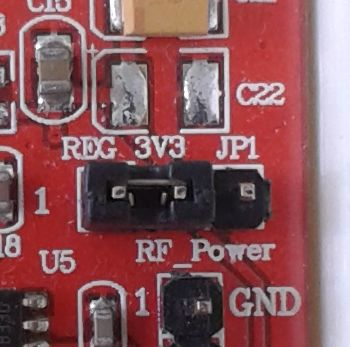
\includegraphics [width=4cm]{jumper_active.jpg} 
 \caption{M24LR board jumper position}
\end{figure}

With this setup you use an external power source. You can therefor use the JTAG pins in the field "`CN1"', which can be found at this position:

\begin{figure}[H]

 \centering
 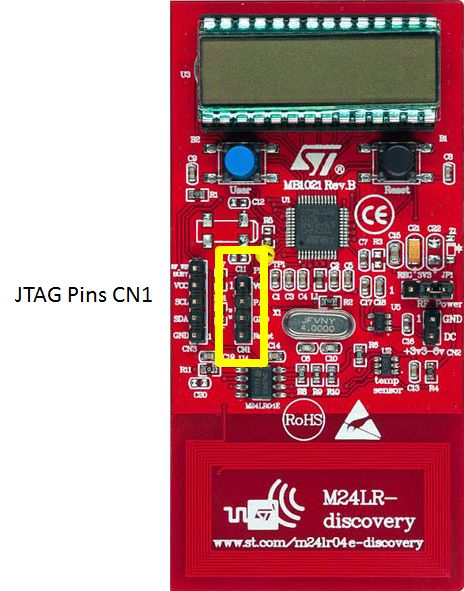
\includegraphics [width=5cm]{JTAG_CN1.jpg} 
 \caption{M24LR board jumper position}
\end{figure}

You have to make sure that the first pin of the JTAG cable is connected to the pin "`VCC"'. The first pin of the cable is marked with a red color. The JTAG cable has to be connected to the "`ST-Link/V2 debugger"'. This device is also needed to program or debug the microcontroller. Although the debugger is connected via USB to the computer it will not provide energy for the microcontroller. Therefor you have to connect the 20 pin JTAG cable from the debugger to the green "`RF transceiver Demonstration Board"'. This board is then connect via USB to the computer. With this connection the combination of debugger and demonstration board will work as a power supply. The overall connection of cables will look like this:

\begin{figure}[H]

 \centering
 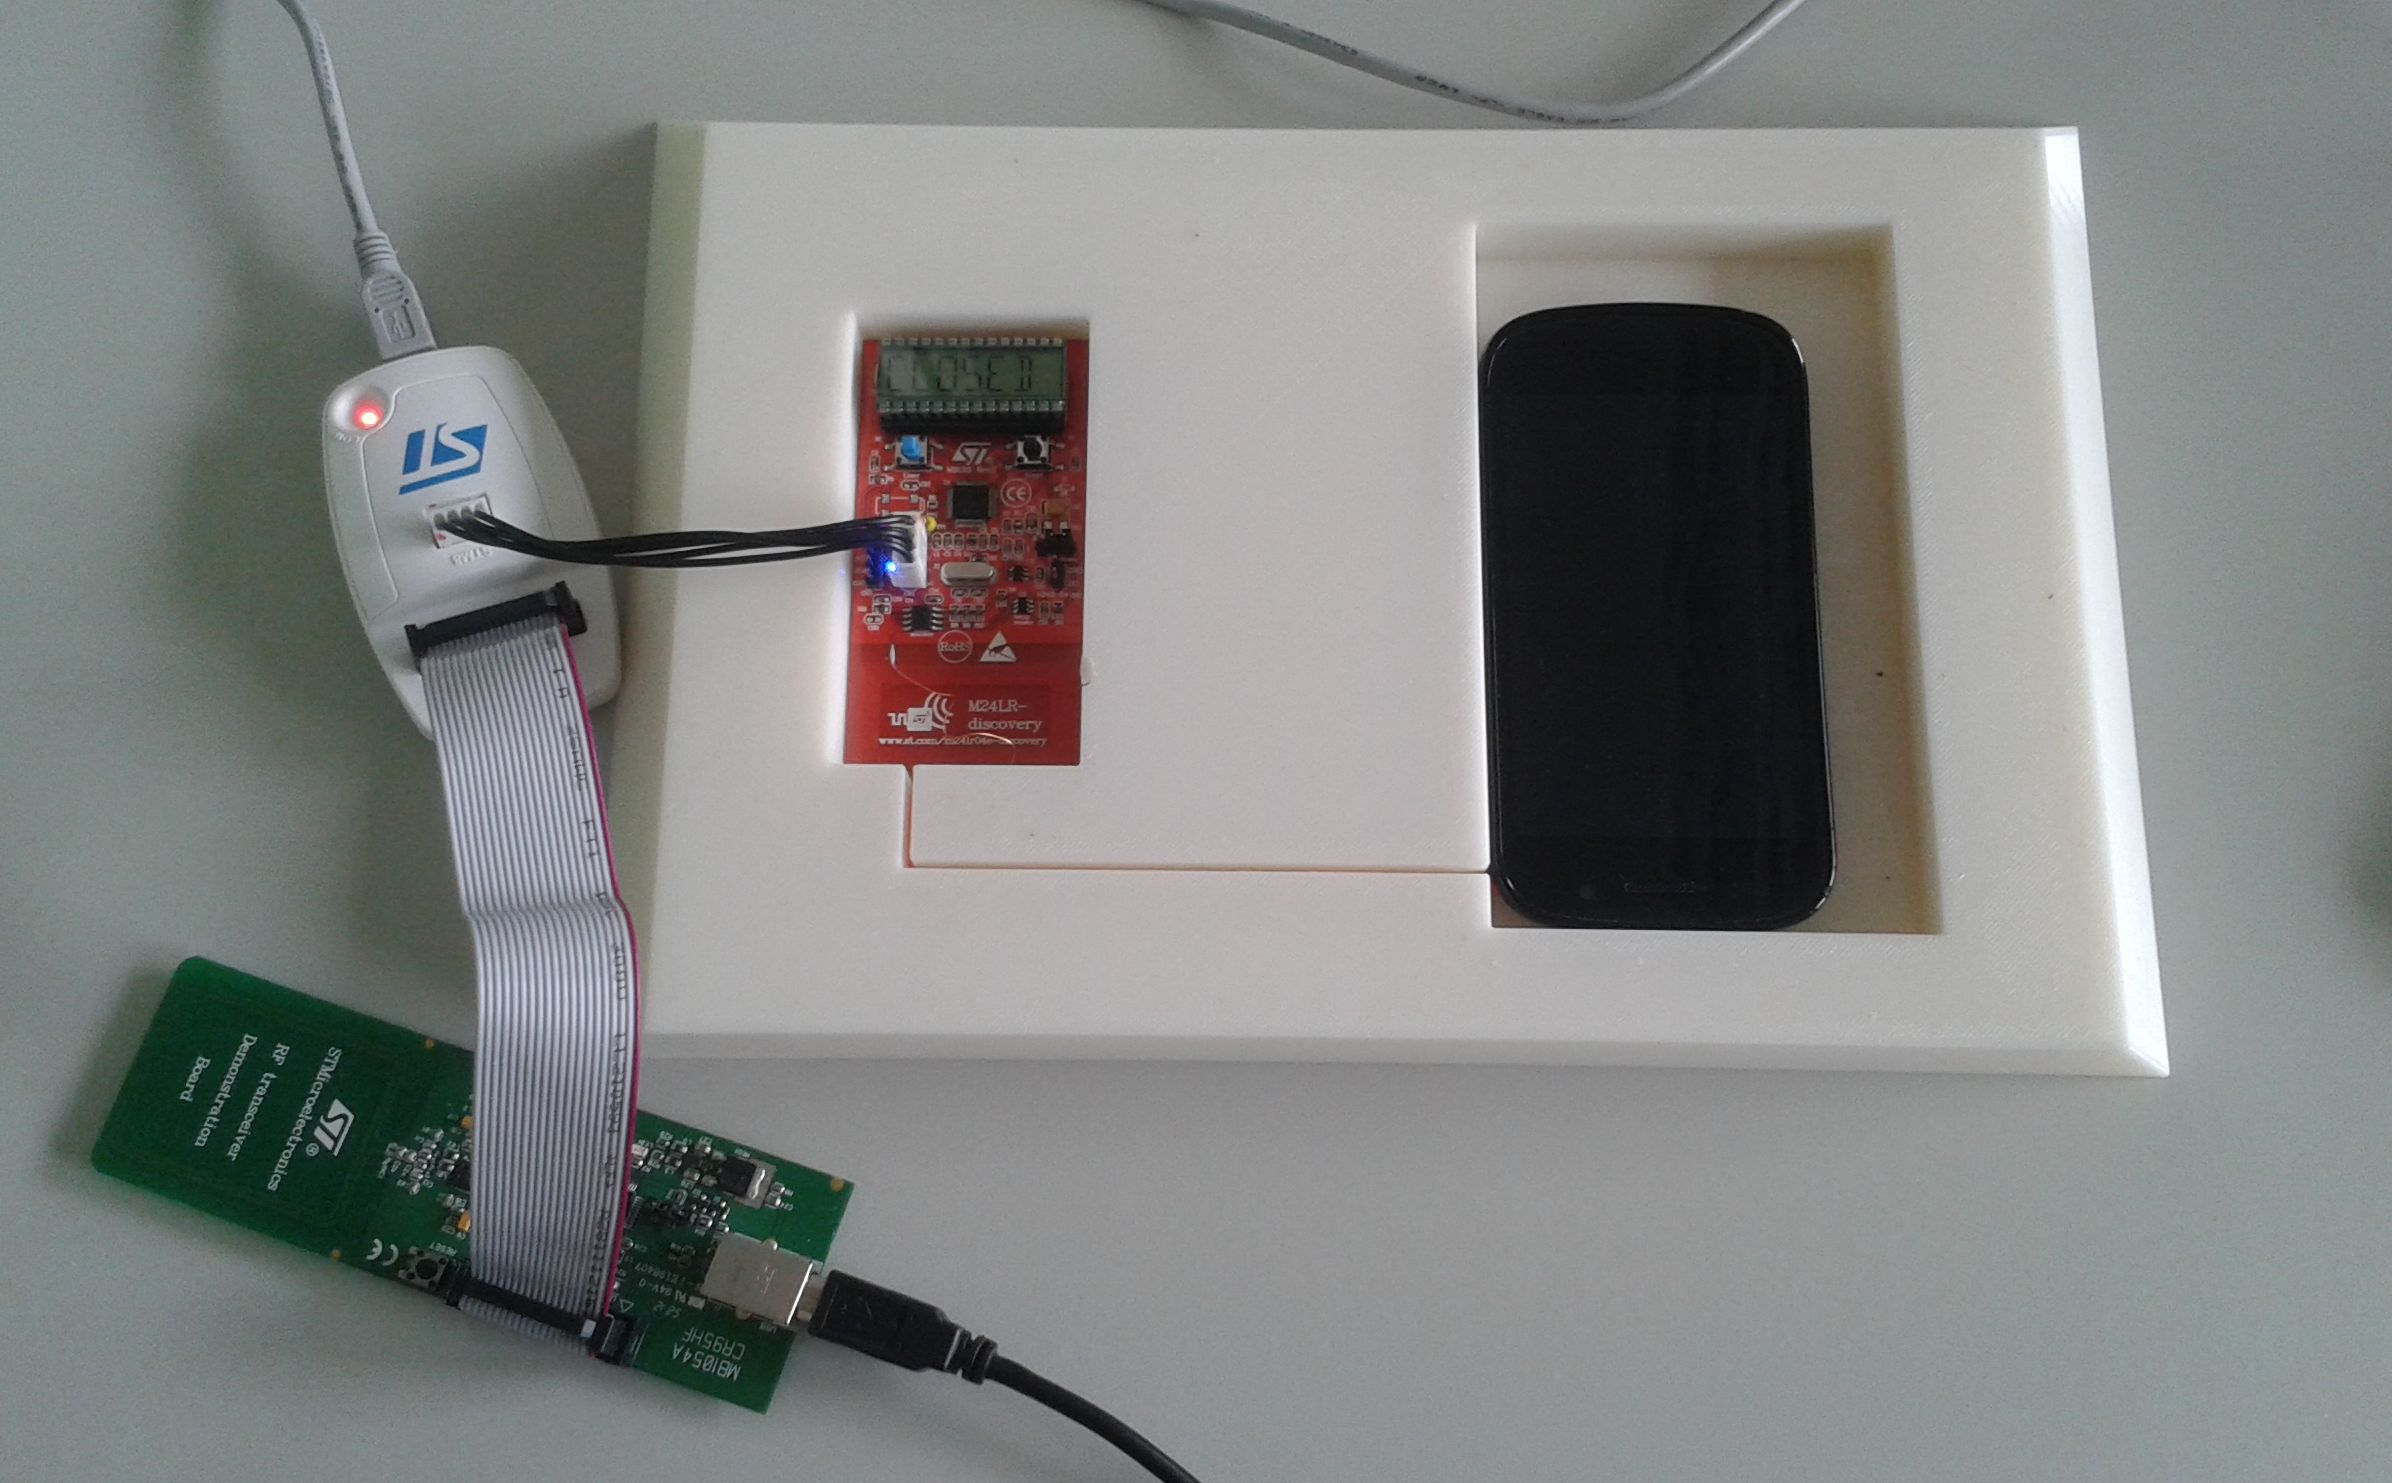
\includegraphics [width=15cm]{hardwaresetup.jpg} 
 \caption{Overall hardware setup}
\end{figure}

\subsubsection{How to setup ST software tools }
If you want to debug or program the microcontroller you can use the tools from ST Microelectronics. To compile your code and to debug the microcontroller you have to use the "`ST Visual Develop"' and to program it you have to use the tool "`ST Visual Programmer"'. You can get both tools from the ST Microelectronics homepage or at the folloing link:\\
Visual Develop: \url{http://www.st.com/web/catalog/tools/FM147/CL1794/SC1808/SS1767/PF210567}\\
Visual Programmer: \url{http://www.st.com/web/en/catalog/tools/PF210568}\\

You also need the "`FREE stm8 32k"' compiler from the company COSMIC. You have to register at their homepage to get a year free license. This can be done at the following link:\\
STM8 32K Comsic compiler: \url{http://www.cosmicsoftware.com/download\_stm8\_32k.php}\\

So after you set up the toolchain you can start the tool ST Visual Develop. After you started it go to File-->Open Workspace. The file you have to open has the ending "`*.stw"'. The file you are looking is this one:

\begin{figure}[H]

 \centering
 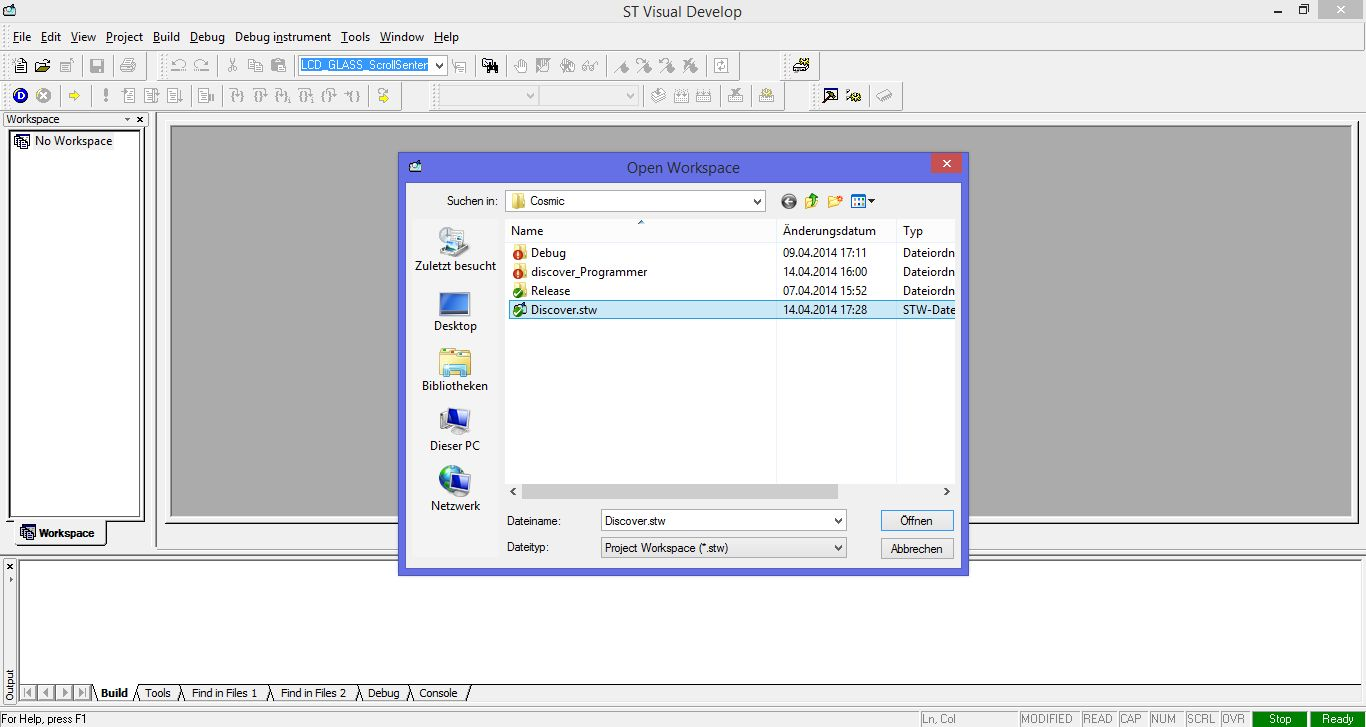
\includegraphics [width=15cm]{STVD_project.jpg} 
 \caption{Overall hardware setup}
\end{figure}

After this you can compile and build the code. Therefore go to Build-->Build or use the hotkey F7.

To program the microcontroller you have to go to Tools--> Programmer. In the next window the settings should look like this:

\begin{figure}[H]

 \centering
 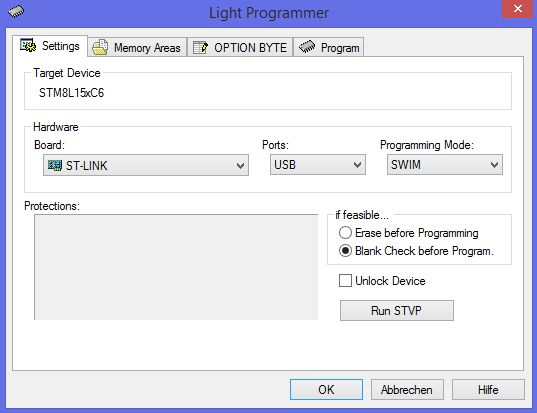
\includegraphics [width=7cm]{programmersettings.jpg} 
 \caption{Overall hardware setup}
\end{figure}

After this start the programmer by clicking on the button "`Run STVP"' and continue with "`Yes"'. The ST Visual Programmer will now open with the right settings of the project. To start the programming go to Program-->Current tab. After the programming is finished you will get the following messages:

\begin{lstlisting}
> Programming  PROGRAM MEMORY area...
Cut Version and Revision of device: 2.0
< PROGRAM MEMORY programming completed.
> Verifying PROGRAM MEMORY area...
Cut Version and Revision of device: 2.0
< PROGRAM MEMORY successfully verified.
\end{lstlisting}

To debug you code on the microcontroller you have to go to Debug-->Start Debugging. However if you are using Windows8 you might get the following error message:\\
** Connection error (usb://usb): gdi-error [40201]: can't access configuration database\\

To avoid this you have the run the file called "`ST Toolset.msi"' in the directory "`<Program Files (x86)>/STMicroelectronics/st\_toolset/stvd/dao/"'. This will solve the problem.

\subsubsection{Running Source Code}

After entering the state machine of this project in the main function, the state machine will in the end enter a state called "`STATE\_CHECKNDEFMESSAGE"'. In this state the received data from the NFC antenna will be interpreted. But first off all in the function below the length of the received message will be checked. The length has to be exactly 5. This is because the message starts with a \$ sign followed by 4 digits of numbers.

\begin{lstlisting}[language=c]
static uint8_t Check_Code_Length(void)
{
  if(CodeLength == 0x05)
  {
  	return SUCCESS;
  }
  else return ERROR;
}
\end{lstlisting}

After the length of the message was checked, you check the variable "`EE\_Buf\_Flag[0]"'. If this variable is equal to 0x00 the microcontroller is in the open state. If it is equal to 0xFF it is in the closed state.
Closed means that the pin is locked and you have to enter the right pin to unlock it. After the right pin is entered the microcontroller switches to the open state, where you can enter a new pin. This pin is then stored in the EEPROM so that it will be still available after restarting the microcontroller.
When the microcontroller writes the new pin into the EEPROM, which happens in the function "`static void Copy\_Units\_in\_other\_memory(void)"' the program checks if the received numbers are really numbers. 

\begin{lstlisting}[language=c]
if(EE_Buffer_2[0] < 0x30 || EE_Buffer_2[0] > 0x39)
{
  ...
}
etc...
\end{lstlisting}

If at least one digit of the NFC message contains no number or wasnt received correctly the LCD display will show the message "`EIT"'.


\subsubsection{MAKE File}
Another part of the project was to create a MAKE file. Therefor I created a batch file to run the MAKE file. The batch file looks like this:

\begin{lstlisting}
set MAKE_MODE=DOS
del /s /q %CD%\makeout\*
rmdir /s /p %CD%\makeout
mkdir %CD%\makeout
make -fMakefile
pause
\end{lstlisting}

The command "`\%CD\%"' means "`current directory"' and the command del, rmdir and mkdir will first delete all files inside of the directory "`makeout"', then delete the directory itself and afterwards recreate it. The command line "`make -fMakefile"' will run the MAKE file with the name "`Makefile"'. To ensure that this command line works, you have to ad the path of make.exe of your GNU MAKE in the PATH variable of windows.\\

The MAKE file is not completed yet. The compiling of the main.c in the directory of the Make file is working. And a template of the creation of the s19 file exists. But there was a problem regarding the access to the directory "`makeout"'. This has to be a problem with rights in windows. For more compiler options and to see how to write MAKE files you have to use the compiler handbook and the GNU Make documentation.

%---------------------------------------------------- New Page -------------------------------------------------
\newpage
\section{Smartphone Bluetooth Device}

This chapter will provide information on the Bluetooth, as well as information to the android application and overall project. The target of the project is to establish a connection between a smartphone and a microcontroller via bluetooth. This is done with a CANblue II device from the company IXXAT Automation GmbH. This device is connected to the microcontroller via CAN and converts the received and send messages into Bluetooth signals. The smartphone used in this project is the "`Google Nexus S"'.

\begin{figure}[H]

 \centering
 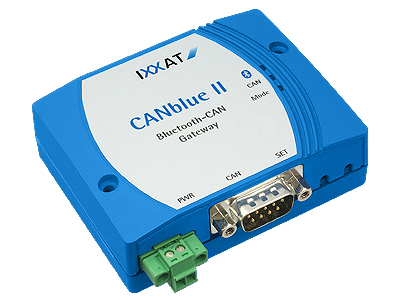
\includegraphics [width=7cm]{interface-canblue-ii.jpg} % You can use this if the picture is in the same folder as the .tex file. Otherwise see above
 \caption{CANBlue II\cite{cite8}}
\end{figure}


%---------------------------------------------------- New Page -------------------------------------------------
\newpage

\subsection{Bluetooth}

Bluetooth is a wireless technology standard to exchange data over short distances. It was originally invented by the company Ericsson in 1994. Today the standard is managed by the Bluetooth Special Interest Group (SIG). To the group belong more than 20000 member companies of the area of telecommunication, computing, networking, and consumer electronics.\\
Bluetooth was planned to be a wireless alternative to RS-232 connections. However today Bluetooth is used to exchange data and in the automotive industrie for hand-free phone systems in infotainment systems. It is also used for audio transmission to external speakers.\cite{cite9}

\subsubsection{Technical Data}
Bluetooth uses a frequency band between 2.4 and 2.485 GHz. The data rate depends on the Bluetooth version that is used:

\begin{itemize} 
\item Version 1.2: 1 MBit/s
\item Version 2.0: 3 MBit/s
\item Version 3.0: 24 MBit/s
\item Version 4.0: 24 MBit/s 
\end{itemize}

The modulation of the radio frequent waves also depend on the version. Up to version 1.2 only the Frequency Shift Keying was used. This means that a higher frequency means a digital 1 and a lower frequency a digital 0:

 
\begin{figure}[H]

 \centering
 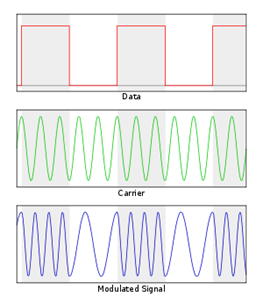
\includegraphics [width=7cm]{fsk.png} 
 \caption{Frequency Shift Keying\cite{cite11}}
\end{figure}

To enhance the data at Bluetooth version 2.0 and above the so called Enhanced Data Rate was introduced. To improve the data rate another type of modulation is used. It is a combination of Frequency Shift Keying and Phase Shift Keying

\begin{figure}[H]

 \centering
 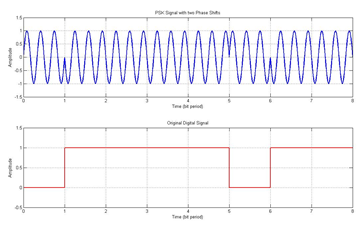
\includegraphics [width=7cm]{psk.png} 
 \caption{Phase Shift Keying\cite{cite12}}
\end{figure}

The even higher bitrate of 24 MBit/s in the Bluetooth versions above 3.0 is realized with a collocated 802.11 link. So the Bluetooth link is only used for negotiation and establishment.

The range of Bluetooth depends on the application that it is used for. The more reliable the connection should be the lower is the maximum range. So the range of Bluetooth connections lie between 10m and 100m.

The Bluetooth protocol is build on a master-slave structure. One master can communicate with up to seven slaves. All devices share the clock of the master. However in a Bluetooth network the master can change while the connection is established.\cite{cite9}

\subsection{NFC Tag to pair Bluetooth Device}

The pairing is one of the essential features of the Bluetooth. There are a few reasons why pairing is useful:
\begin{itemize} 
\item Private data is exchanged in Bluetooth, e.g. phone numbers at infotainment system
\item For security reasons it is necessary to recognize specific devices that are allowed to connect to the Bluetooth device
\item For comfortable reason: After pairing the Bluetooth device will establish a connection every time the other device enters the range of Bluetooth
\end{itemize}

In this project the pairing with the CANBlue II device is done by a NFC tag. The android app "`NFC TagWriter by NXP"' is used to write via NFC on the NFC tag. This app has several possibilities to write content on the tag. This is for example:

\begin{itemize} 
\item Plain Text
\item Start of an installed android application
\item Pairing with Bluetooth device
\end{itemize} 

To create content on a tag you have to click on "`Create, write and store"'.

\begin{figure}[H]

 \centering
 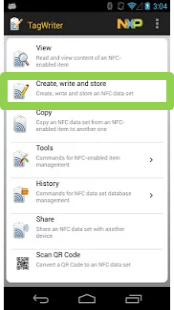
\includegraphics [width=4cm]{tagwriter.png} 
 \caption{Tagwriter App\cite{cite13}}
\end{figure}

After that you have to click on Bluetooth and then follow the instructions. Each Bluetooth device has its very own MAC address. In this project the CANBlue II device has the MAC address "`00:12:F3:1A:C8:9E"'. After clicking on the next button, you have to put the NFC tag under the NFC antenna and the content will be stored on the tag.

\begin{figure}[H]

 \centering
 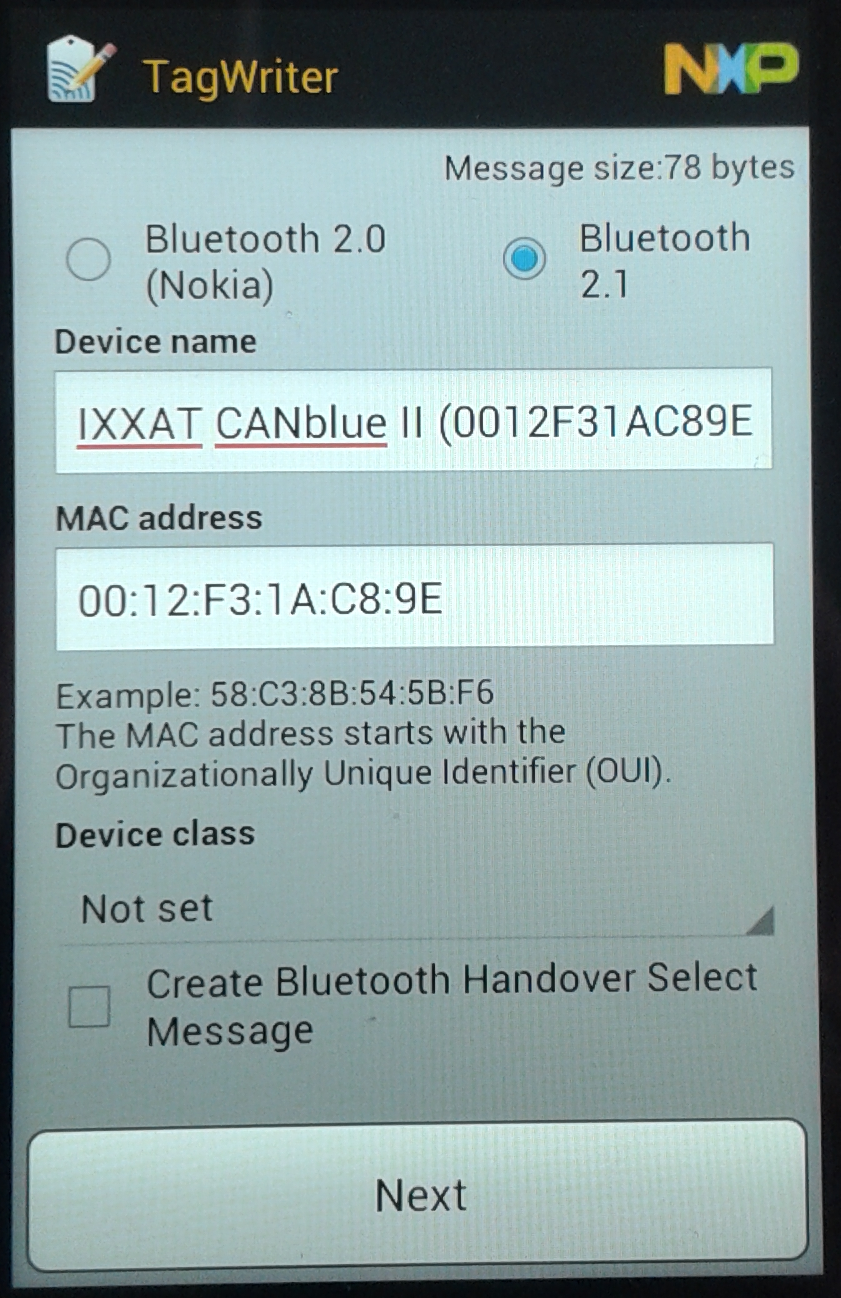
\includegraphics [width=4cm]{bluetooth.png} 
 \caption{Tagwriter App Bluetooth}
\end{figure}



\subsection{Android Application}

\subsubsection{How to setup tools}
For the programming of the android application the tool Eclipse with the Android Developer Tool Bundle was used. You can get the tool at\\ \url{http://developer.android.com/sdk/index.html}.

To work with the project you have to import it. Therefor go to File-->Import.... After that choose "`Existing Projects into Workspace"' and click on Next. Choose the directory where the project is, select the project and click on finish.
Because the project is also build for android version below 3.0 you have to import a support library. This can be found at "`../adt-bundle-windows-x86\_64-20130522/sdk/extras/android/support/v7/appcompat"'.

After the projects are imported rightclick on it and choose "`Properties"'. Make sure that the following settings are selected. Additionally make sure that at the tab "`Java Build Path-->Order and Export"' the library "`API\_ADK.jar"' is on top of the list.

\begin{figure}[H]

 \centering
 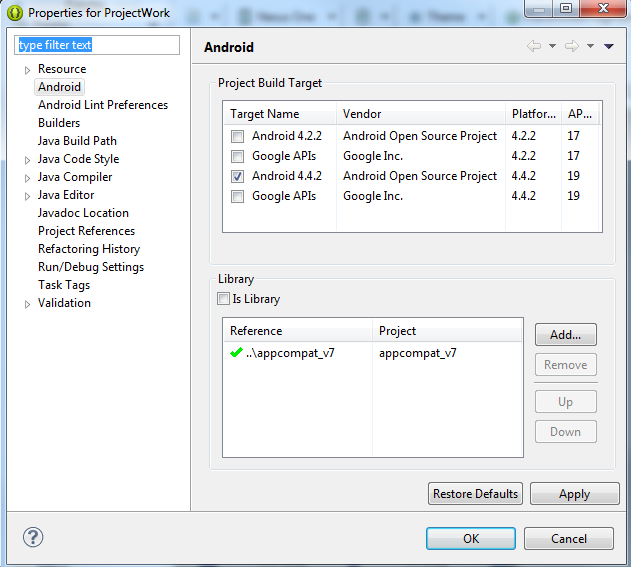
\includegraphics [width=10cm]{properties.png} 
 \caption{Tagwriter App Bluetooth}
\end{figure}

\newpage

\subsubsection{Application}

After starting the application the first screen looks like this:

\begin{figure}[H]

 \centering
 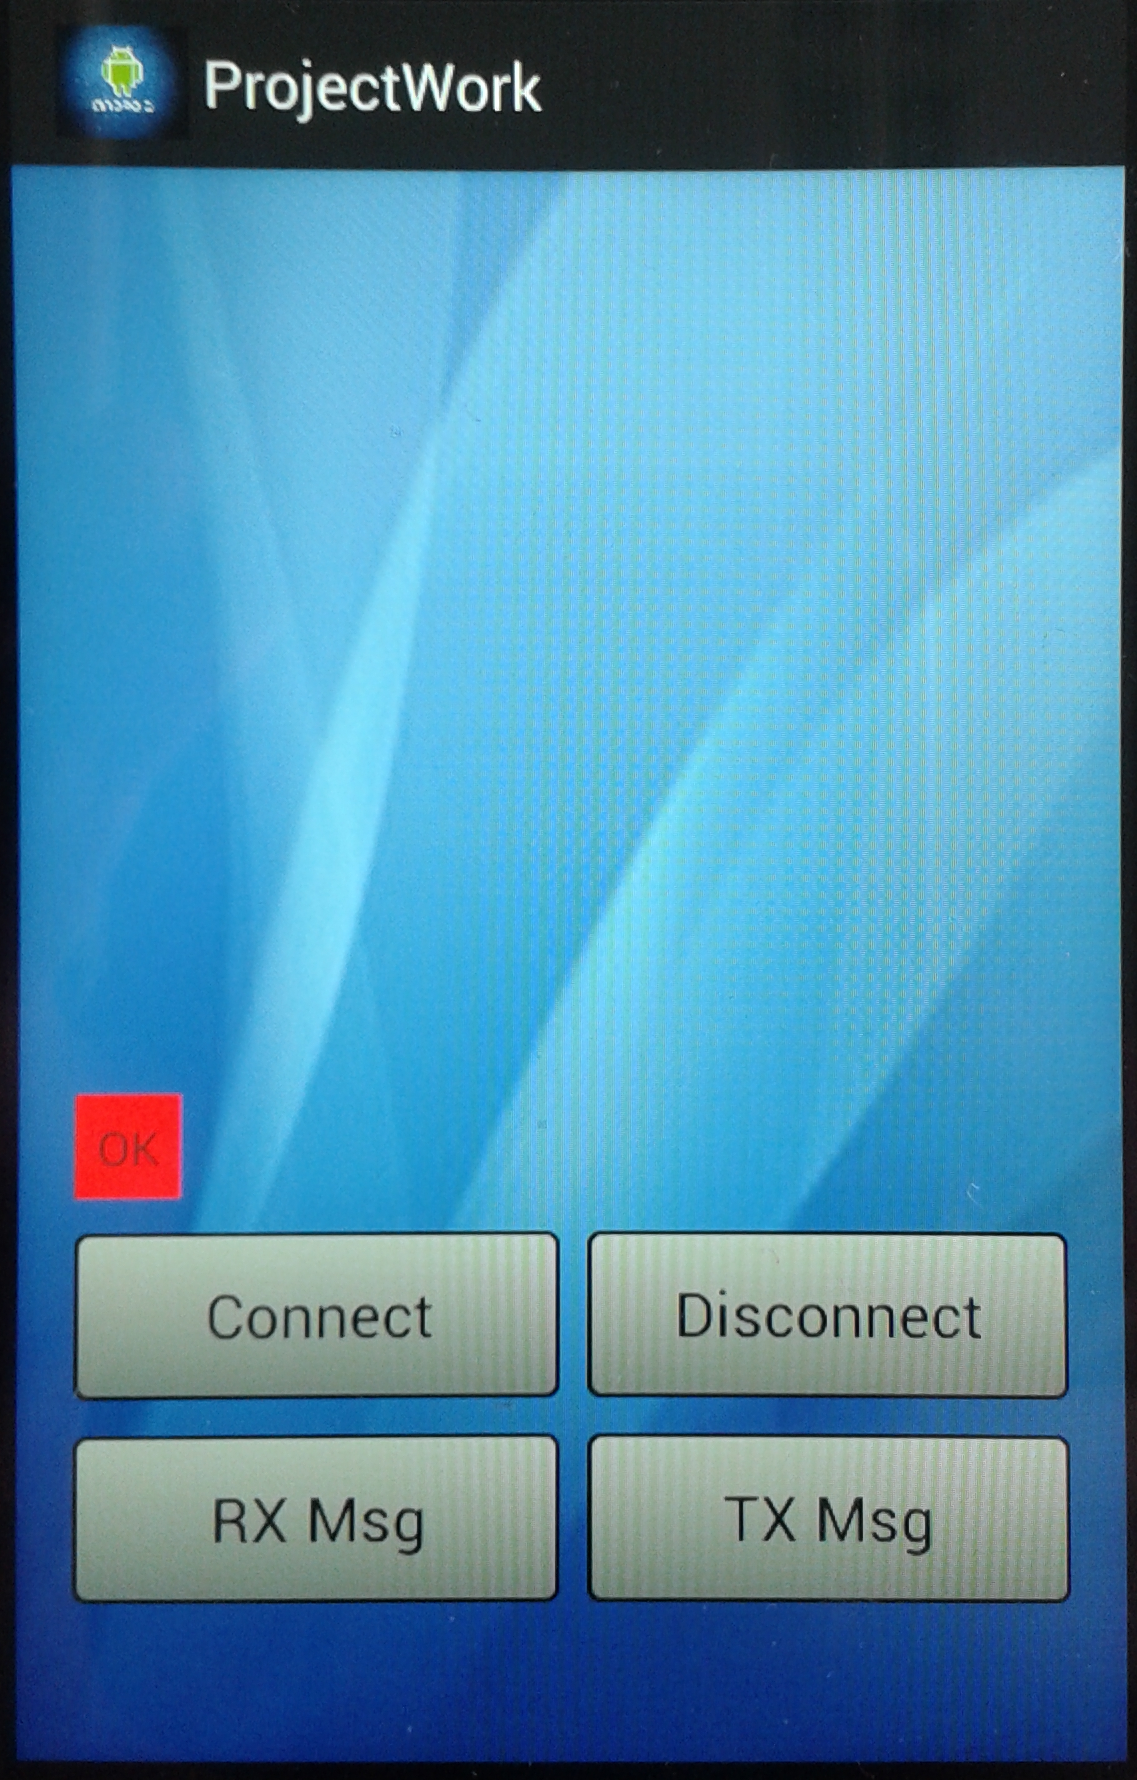
\includegraphics [width=3cm]{startscreen.png} 
 \caption{Tagwriter App Bluetooth}
\end{figure}

It consists of 4 buttons a textbox. The functions behind the buttons can be found in the file MainActivity.java and are the following:

\begin{itemize} 
\item Connect --> public void connectButton(View view)\{\}
\item Disonnect --> public void disconnectButton(View view)\{\}
\item RX Msg --> public void txButton(View view)\{\}
\item TX Msg --> public void rxButton(View view)\{\}
\end{itemize} 

The connect button starts the connection to the CANBlue II device. After the connection a few information will be displayed in the textbox:
\begin{figure}[H]

 \centering
 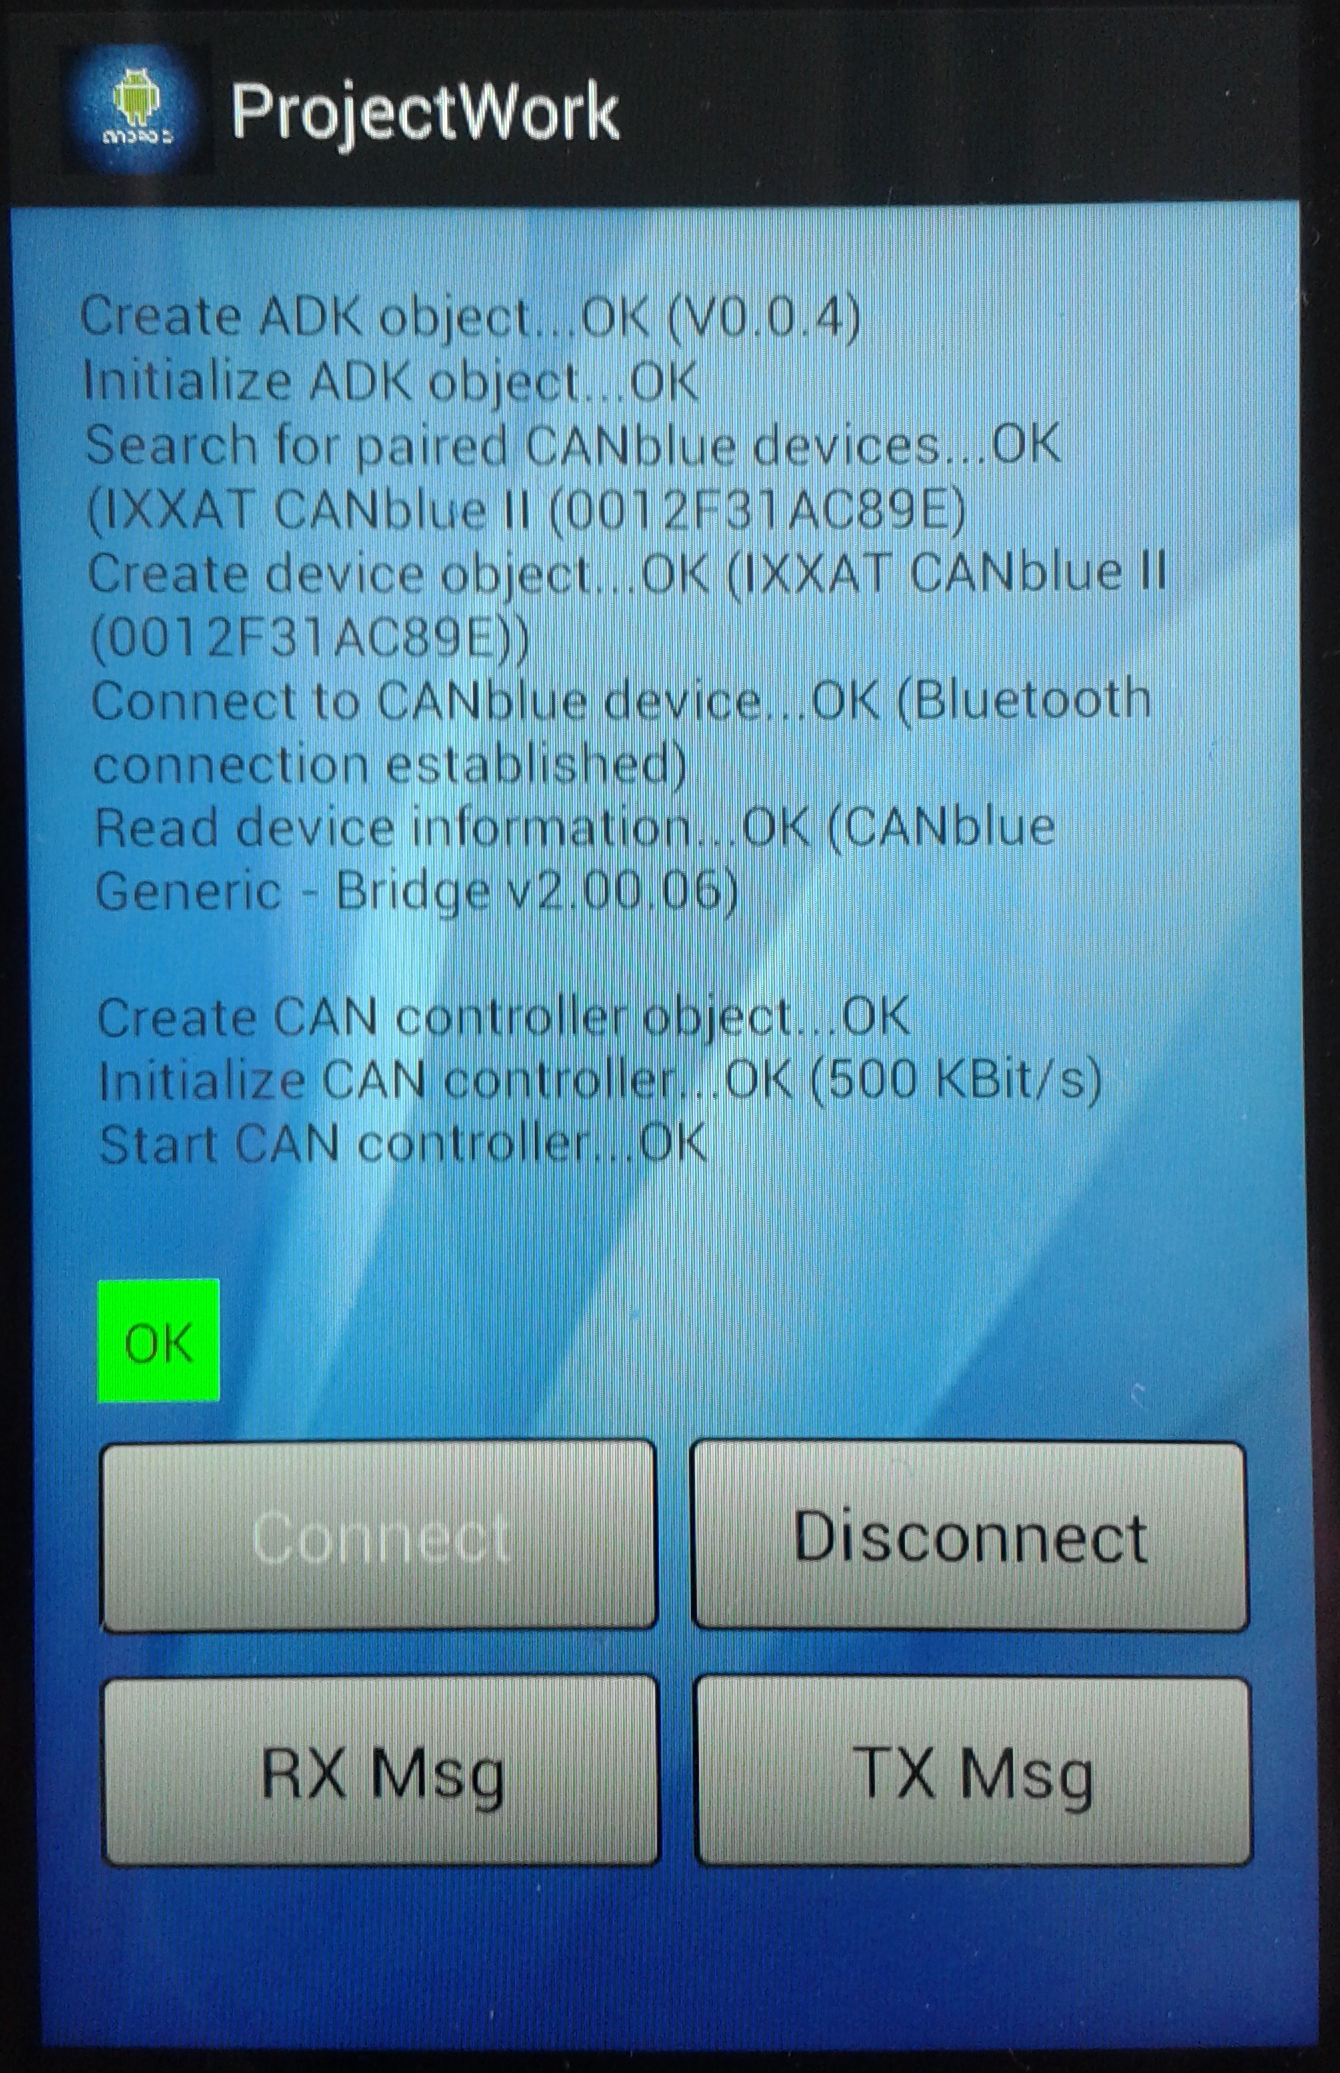
\includegraphics [width=4cm]{connectbutton.png} 
 \caption{Tagwriter App Bluetooth}
\end{figure}

With the disconnect button the smartphone will disconnect from the CANBlue II device. To disconnect the controller first of all the controller is stopped and  deinitialized. After that the device is disconnected and at the end the ADK object is deinitialized. After each step the return code is checked if it was successful.


\begin{lstlisting}[language=java]
public void disconnectButton(View view)
{				
  if(demoController != null && ADK != null)
  {
    if(demoController.stopController() == ReturnCode.SUCCESS)
    {
      textview.setText("StopController successful\n");
      if(demoController.deinitializeController() == ReturnCode.SUCCESS)
      {
        textview.append("Deinitialize Controller successful\n");
        if(demoDevice.disconnectDevice() == ReturnCode.SUCCESS)
        {
          textview.append("Deinitialize device successful\n");
          if(ADK.deinitializeADK() == ReturnCode.SUCCESS)
          {
            TextView textview2 = (TextView) findViewById(R.id.textView2);
            textview2.setBackgroundColor(getResources().getColor(R.color.red));
            
            Button btn=(Button)findViewById(R.id.button1);
            btn.setEnabled(true);
            
            btn = (Button) findViewById(R.id.button4);
            btn.setEnabled(false);
            
            textview.append("Deinitialize ADK successful\n");
          }
        }
      }
    }
  }
}	
\end{lstlisting}


The TX button will go to the next activity where the messages can be send to the device. The activity looks like this: 

\begin{figure}[H]

 \centering
 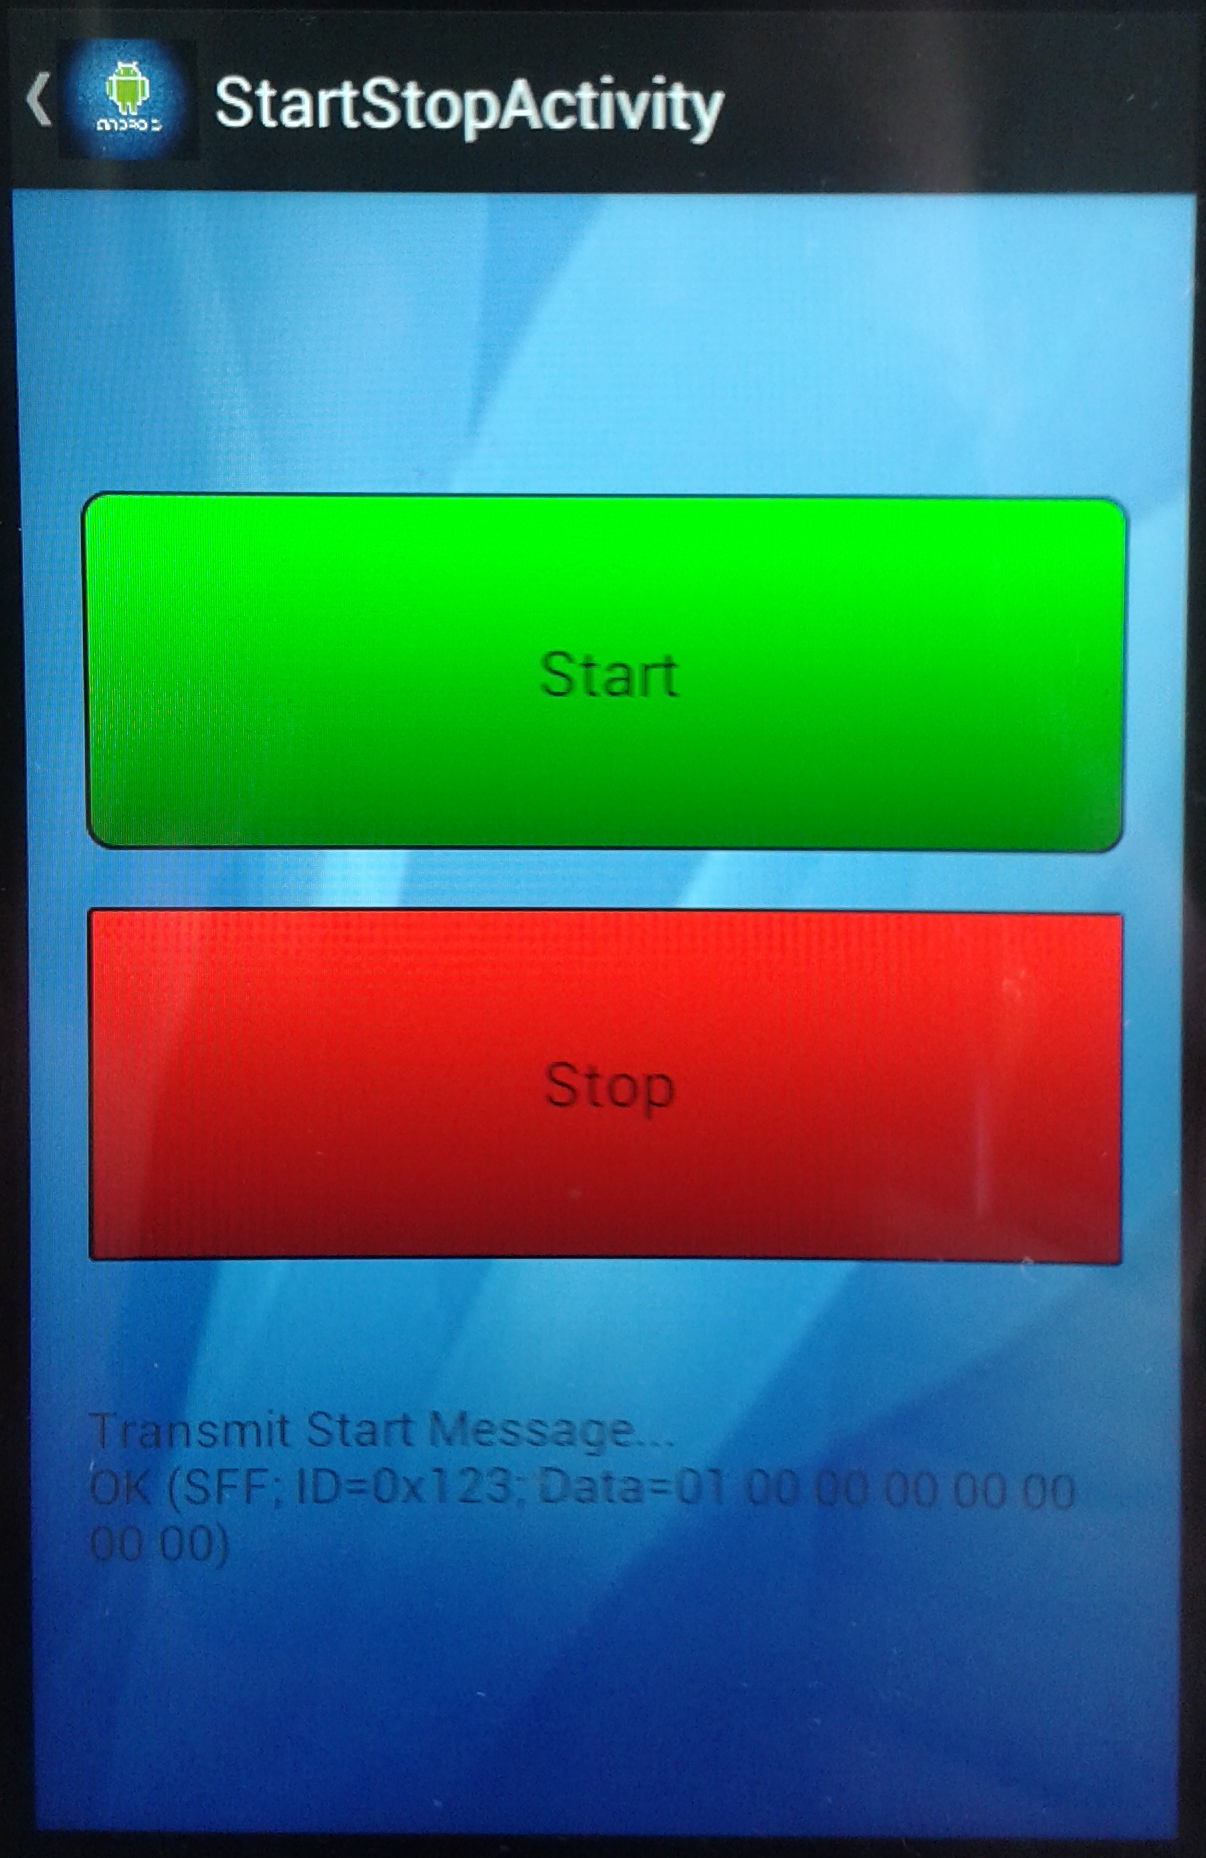
\includegraphics [width=4cm]{startstop.png} 
 \caption{Tagwriter App Bluetooth}
\end{figure}

On this activity there are two buttons. One button is to send a CAN message to start the actuator which is connected to the Arduino microcontroller. To do that before sending the message the frameformat, frametype, datalength, messageID and data payload have to be set. In this project we use a standard frame for the format, a data frame for the frametype, a data length of 8 byte and the message ID 0x123. The following code is used for that:

\begin{lstlisting}[language=java]       
 demoTxMsg.frameFormat = ConstantList.STANDARD_FRAME;
 demoTxMsg.frameType = ConstantList.DATA_FRAME;
 demoTxMsg.dataLength = (byte) 8;
 demoTxMsg.messageID = 0x123;
       
 /* set the data of the CAN Message */
 demoTxMsg.data[0] = 0x01;
 demoTxMsg.data[1] = 0x00;
 demoTxMsg.data[2] = 0x00;
 demoTxMsg.data[3] = 0x00;
 demoTxMsg.data[4] = 0x00;
 demoTxMsg.data[5] = 0x00;
 demoTxMsg.data[6] = 0x00;
 demoTxMsg.data[7] = 0x00;
\end{lstlisting}

This code can be found in the function "public void startClick(View view)" in the file StartStopActivity.java. The sending of the message is realized with this function:

\begin{lstlisting}[language=java]  
MainActivity.demoController.transmitMessage(demoTxMsg, ConstantList.BINARY_FORMAT);
\end{lstlisting}

To stop the actuator the first byte of the CAN message payload has to be change to 0x00. This is done in the function "public void stopClick(View view)"


There also exists an activity for receiving and showing messages. But due to the lack of time the reception of messages is not working correctly. The error has to be somewhere in the function "protected void onCreate(Bundle savedInstanceState)" in the file RxActivity.java.

%----------------------------------------------------------------------------------------
%	REFERENCE LIST
%----------------------------------------------------------------------------------------
\newpage
\begin{thebibliography}{99} % Bibliography - this is intentionally simple in this template

\bibitem{cite1} http://en.wikipedia.org/wiki/Near\_Field\_Communication
\bibitem{cite2} http://nfc-forum.org/about-us/our-members/
\bibitem{cite3} http://www.nfcworld.com/2010/12/16/35503/nexus-s-teardown-how-nfc-fits-inside-the-new-google-phone/
\bibitem{cite4} ac\_t3\_bluetooth.pdf, Prof. Dr.-Ing. Harald Melcher
\bibitem{cite5} http://www.mathworks.com/matlabcentral/fx\_files/30580/1/ASK.jpg
\bibitem{cite6} http://www.droid-life.com/wp-content/uploads/2013/05/EAD-X11SWE\_02.png
\bibitem{cite7} http://www.st.com/web/en/catalog/tools/FM116/SC1444/PF253360
\bibitem{cite8} http://www.ixxat.de/canblue\_2\_de.html
\bibitem{cite9} http://en.wikipedia.org/wiki/Bluetooth
\bibitem{cite10} https://play.google.com/store/apps/details?id=com.nfc.apps\&hl=de
\bibitem{cite11} http://en.wikipedia.org/wiki/Frequency\_shift\_keying
\bibitem{cite12} http://www.zhihuishi.com/Image.ashx?ID=8307
\bibitem{cite13} https://play.google.com/store/apps/details?id=com.nxp.nfc.tagwriter\&hl=de


\end{thebibliography}

%----------------------------------------------------------------------------------------

%\end{multicols}

\end{document}
